\chapter{Bass-Serre-Theorie}

% =============
\section{Die Fundamentalgruppe eines Graphen}\label{sec_FG}

\DB Es sei $\GR$ ein zusammenhängender Graph und $p\in E(\GR)$.
\begin{enumerate}
\item $\pi_1(\GR,p)$ sei die Menge der stachelfreien geschlossenen
Wege in $\GR$ mit Anfangs- und Endpunkt $p$.
\item Für $w_1, w_2\in \pi_1(\GR,p)$ sei $w_1\cdot w_2$ der
Weg, den man nach dem Entfernen aller Stachel des aus $w_1$ und $w_2$
zusammengesetzen Weges erhält.
\item Mit dieser Verknüpfung ist $\pi_1(\GR,p)$ eine Gruppe.
Sie heißt \emph{Fundamentalgruppe}\index{Fundamentalgruppe}\index{Gruppe!Fundamental-}\index{$\pi_1(\GR,p)$, $\pi_1(\GR)$}
von $\GR$ (bzgl. $p$).
\item Für jedes $q\in E(\GR)$ ist $\pi_1(\GR,q)\cong\pi_1(\GR,p)$.
Daher können wir auch $\pi_1(\GR)$ schreiben.
\end{enumerate}
\bew
\begin{itemize}
\item[3.] Das neutrale Element ist der Weg der Länge $0$.
Zu $w=(k_1,\ldots,k_n)$ ist
$\bar{w}=(\bar{k}_n,\ldots,\bar{k}_1)$ invers.

Die Zeichnung veranschaulicht, wie beim Zusammensetzen zweier
stachelfreier Wege neue Stachel autreten können.
\begin{center}
	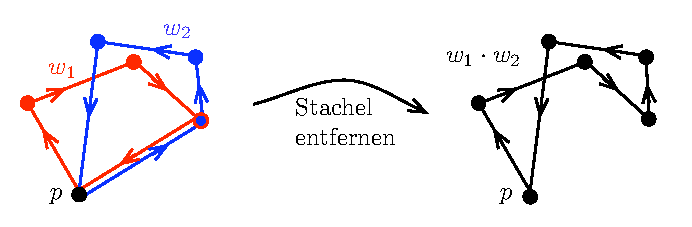
\includegraphics{grugraImages/w1w2}
\end{center}
Hat ein zusammengesetzter Weg $w=(k_1,\ldots,k_n)$ einen Stachel,
so muss $\bar{k}_i=k_{i+1}$ für ein $i$ gelten.
Setze $w^{(1)}:=(k_1,\ldots,k_{i-1},k_{i+2},\ldots,k_n)$ und
wiederholen dieses Vorgehen solange, bis alle Stacheln entfernt sind.
Wir bemerken, dass dies zu einem eindeutigen stachelfreien Weg führt.
Daraus folgt die Wohldefiniertheit der Verknüpfung und ebenso die
Assoziativität.
\item[4.] Es sei $v$ ein Weg in $\GR$ von $p$ nach $q$. Dann ist
\[
\phi:\pi_1(\GR,q)\Ra\pi_1(\GR,p),\quad
w\mapsto vw\bar{v}
\]
ein Gruppenhomorphismus, denn
\[
\phi(w_1 w_2) = v w_1 w_2 \bar{v}
=v w_1 \bar{v} v w_2 \bar{v}
=\phi(w_1)\phi(w_2).
\]
Da es offensichtlich eine Umkehrung gibt, ist $\phi$ bijektiv.
\qed
\end{itemize}

\BSP\
\begin{enumerate}
\item Ist $\GR$ ein Baum, so ist $\pi_1(\GR,p)=\{1\}$.
\item Es sei
\begin{center}
	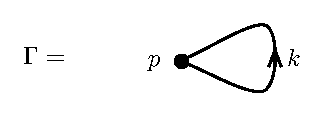
\includegraphics{grugraImages/pi1Z}
\end{center}
Die Gruppe $\pi_1(\GR,p)$ besteht aus dem Weg der Länge $0$
und aus den Wegen, die durch
$n$-faches Durchlaufen von $k$ oder $n$-faches Durchlaufen von
$\bar{k}$ entstehen. Daher ist $\pi_1(\GR,p)\cong\ZZ$.
\item Es sei
\begin{center}
	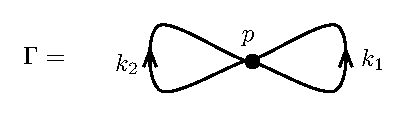
\includegraphics{grugraImages/pi1F2}
\end{center}
In diesem Fall ist $\pi_1(\GR,p)=F_2$.
\end{enumerate}

\PROP\label{prop_zusfrei}
Für jeden zusammenhängende Graphen $\GR$ ist $\pi_1(\GR)$
eine freie Gruppe vom Rang $g(\GR)$.

\bew Für den Fall, dass $\GR$ hat nur eine Ecke hat:\\
Die Kanten $k\in K(\GR)$ können als Elemente von $\pi_1(\GR)$
aufgefasst werden. Für $k\in K(\GR)$ ist $\bar{k}$ das inverse
Element. Die stachelfreien Wege in $\GR$ entsprechen bijektiv
den Kantenfolgen der Form
\[
k_1^{\eps_1},\ldots,k_n^{\eps_n}
\]
mit $n\geq 0$, $\eps_i=\pm 1$ und
$k_{i+1}^{\eps_{i+1}}\neq k_i^{-\eps_i}$.
Diese Stellen aber genau die reduzierten Worte in
$F(K(\GR)^+)$ dar, wobei $K(\GR)^+$ eine Orientierung von
$\GR$ ist.

Nun der Beweis für den allgemeinen Fall:\\
Es sei $T$ ein aufspannender Teilbaum
von $\GR$ und $\GR':=\GR/T$. Nach Bemerkung \ref{bem_GZ}(2) ist
$g(\GR')=g(\GR)$. Zusammen mit dem Fall für eine Ecke genügt es
nun zu zeigen, dass $\pi_1(\GR')\cong\pi_1(\GR)$ ist.
\qed

\BEM Es sei $\GR$ ein zusammenhängender Graph, $Z$ ein Teilgraph
$z\in Z$.
Dann gibt es einen surjektiven Homomorphismus
$\phi_Z:\pi_1(\GR,z)\Ra\pi_1(\GR/Z,Z)$, dessen Kern die
normale Hülle von $\pi_1(Z,z)$ ist, d.h.
\[
\K{\phi_Z}=\lag\pi_1(Z,z)\rag_{\mathrm{NT}}:=
\bigcap_{\pi_1(Z,z)\subset N \unlhd \pi_1(\GR,z)} N.
\]
\bew Für $w=(k_1,\ldots,k_n)\in\pi(\GR,z)$ sei
$\psi_Z(w)$ der Weg, der durch Streichen alle Kanten in $K(Z)$
entsteht und $\phi_Z(w)$ der Weg, der durch Entfernen aller Stacheln
aus $\psi_Z(w)$ entsteht. Man sieht leicht, dass $\phi_Z$ ein
Gruppenhomomorphismus ist.

$\phi_Z$ ist surjektiv: Fasse $w$ als Weg in $\pi_1(\GR/Z,Z)$ auf.
Dann sind $k_1,\ldots,k_n\in K(\GR)\backslash K(Z)$.
Ist $\ter(k_i)\neq \ini(k_{i+1})$ in $E(\GR)$, so ist
$\ter(k_i)=\ini(k_{i+1})=Z$ in $E(\GR/Z)$.
Da $Z$ zusammenhängend ist, gibt es einen Weg $v_i$ in $Z$ mit
$\ini(v_i)=\ter(k_i)$ und $\ter(v_i)=\ini(k_{i+1})$.
Also ist
\[
\tilde{w}=
(v_0,k_1,v_1,\ldots,k_n,v_n) \in \pi_1(\GR,z)
\]
ein Weg in $\GR$ mit $\phi_Z(\tilde{w})=w$
(dabei dürfen die Wege $v_i$ die Länge $0$ haben und bei Bedarf
sei $v_0$ ein Weg in $Z$ von $z$ nach $\ini(k_1)$ und $v_n$ ein
Weg in $Z$ von $\ter(k_n)$ nach $z$).
\begin{center}
	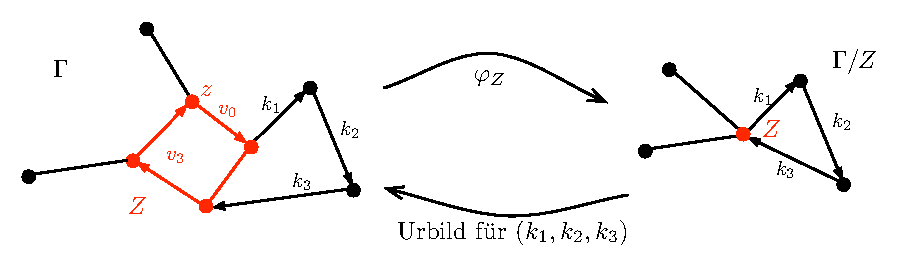
\includegraphics{grugraImages/phiZ}
\end{center}
Offensichtlich liegt $\pi_1(Z,z)$ im Kern von $\phi_Z$. Da der Kern
ein Normalteiler ist, der $\pi_1(Z,z)$ enthält, muss er auch
den Schnitt über alle solchen Normalteiler enthalten,
also $\lag \pi_1(Z,z)\rag_{\mathrm{NT}}\subseteq \K{\phi}$.

Zum Beweis der umgekehrten Inklusionrichtung überlegen wir zuerst,
dass ein Weg $w\in \K{\phi_Z}$ in der Form
\[
v_0 w_1 v_1 w_2 v_2 \cdots w_n v_n
\]
geschrieben werden kann, wobei $v_i$ ein Weg in $Z$ und $w_i$ ein
Weg außerhalb von $Z$ ist (jedoch mit Anfangs und Endpunkt in $Z$).
Es muss $\psi_Z(w)=w_1 w_2 \ldots w_n$ ein Stachel sein.
Wir wählen stachelfreie Wege $u_i\in\pi_1(Z,z)$ von $\ter(w_i)$ nach
$z$ und $u_i'\in\pi_1(Z,z)$ von $\ter(v_i)$ nach $z$.
Dann können wir $w$ schreiben als
\begin{align*}
w &= v_0 w_1 (u_1 u_1^{-1}) v_1 (u_1' u_1'^{-1}) w_2 \cdots \\
&=\ub{v_0 w_1 u_1}{\in \pi_1(\GR,z)}
\ub{u_1^{-1} v_1 u_1'}{\in \pi_1(Z,z)}
\ub{u_1'^{-1} w_1 u_2}{\in \pi_1(\GR,z)} \cdots .
\end{align*}
Wir können also ohne Einschränkung annehmen, dass
$w_i\in\pi_1(\GR,z)$ und $v_i\in\GR(Z,z)$ gilt. Damit erhalten wir
\begin{align*}
w =&
\ub{w_1 v_1 w_1^{-1}}{\lag \pi_1(Z,z)\rag_{\mathrm{NT}}}
\ub{w_1 w_2 v_2 w_2^{-1} w_1^{-1}}{\lag \pi_1(Z,z)\rag_{\mathrm{NT}}}
\ub{w_1 w_2 w_3 v_3 w_3^{-1} w_2^{-1} w_1^{-1}}{\lag \pi_1(Z,z)\rag_{\mathrm{NT}}}\\
&\cdots
\ub{w_1\cdots w_{n-1}\ldots v_1 w_{n-1}^{-1}\cdots w_1^{-1}}{\lag \pi_1(Z,z)\rag_{\mathrm{NT}}}
\cdot
\ub{w_1\cdots w_n}{\text{Stachel}},
\end{align*}
also $w\in\lag \pi_1(Z,z)\rag_{\mathrm{NT}}$.
\qed

\PROP Zu jedem Graphen $\GR$ gibt es einen Baum $X=X_{\GR}$ und eine
freie Aktion von $\pi_1(\GR)$ auf $X$, so dass
$X/\pi_1(\GR)\cong \GR$.

\bew
Es sei $T$ ein maximaler Teilbaum von $\GR$ und $S$ eine Orientierung
von $K(\GR)\backslash K(T)$. Dann ist $\pi_1(\GR)\cong F(S)$
nach Proposition \ref{prop_zusfrei}.

Die Idee, die der folgenden Konstruktion von $X$ zugrunde liegt,
ist es, für jedes Element von $F(S)$ eine Kopie von
$T$ zu erstellen, so dass $F(S)$ frei auf diesen Kopien operieren
kann. Dazu identifizieren wir ein $s\in S$ mit dem Element
von $\pi(\GR)$, dass $s$ enthält und sonst nur Kanten in $T$
(dies ist eindeutig, da $T$ ein Baum ist).
Nun definieren wir $X$ durch
\begin{align*}
E(X) &:= \BCUP{.}{g\in\pi_1(\GR)} g\cdot E(T), \\
K(X) &:= \Bigl(\BCUP{.}{g\in\pi_1(\GR)} g\cdot K(T)\Bigr)
\cup
\Bigl(\BCUP{}{s\in S}\BCUP{}{g\in\pi_1(\GR)} \{gs, g\bar{s} \}\Bigr)
\end{align*}
mit $\ini(gs):=g\ini(s)$, $\ter(gs):=gs\ter(s)$ und entsprechend
für $g\bar{s}$.
$\pi_1(\GR)$ operiert auf $X$ durch Linksmultiplikation.

Es ist $X/\pi_1(\GR)=\GR$ nach Konstruktion. $X$ ist
zusammenhängend, da $S$ die Gruppe $\pi_1(\GR)$ erzeugt
(vgl. Beweis von Proposition \ref{prop_zusfrei}).
Gäbe es Kreise in $X$, so gäbe es ein reduziertes Wort in den
Elementen aus $S$, im Widerspruch dazu, dass die Aktion frei ist.
Somit muss $X$ ein Baum sein.
\qed

\DEF Der Baum $X_{\GR}$ heißt \emph{universelle Überlagerung}\index{universelle Überlagerung} von $\GR$.

\BSP\label{bsp_univ} Es sei
\begin{center}
	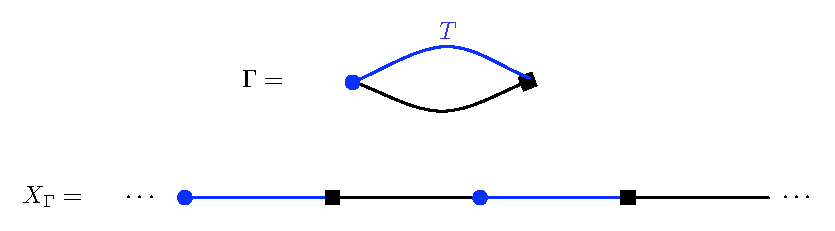
\includegraphics{grugraImages/univ}
\end{center}
$n\in\ZZ=\pi_1(\GR)$ operiert durch Translation um $2n$.

Die hier gegebenen Definitionen der Fundamentalgruppe und der
universellen Überlagerung sind konsistent mit denen aus der
Topologie, wenn wir die Graphen als topologische Teilräume
eines $\RR^n$ auffassen
(vgl. Abschnitte 1.1 und 1.3 in Hatcher \cite{hatcher}).
So entspricht der Graph $\GR$ aus
Beispiel \ref{bsp_univ} dem Einheitskreis $S^1$, dessen
universelle Überlagerung $X_{\GR}$ die reellen Zahlen $\RR$ sind.


% ==================
\section{Freie Gruppen und Amalgame}\label{sec_amal}

Es sei $G$ eine Gruppe und $S$ eine Erzeugermenge von $G$.
Die UAE der freien Gruppen impliziert
$G\cong F(S)/\K{\Phi}$ für den Homomorphismus
$\Phi:F(S)\Ra G$, $s\mapsto s$ (man kann sich $\Phi$ als
\glqq Anwendung der in $G$ gültigen Relationen \grqq\ auf Worte
in $F(S)$ vorstellen).\index{Relationen}

\DEF Es sei $R\subset \K{\Phi}$ mit
$\lag\Phi\rag_{\mathrm{NT}} = \K{\Phi}$. Schreibe
\[
\lag S|R \rag := G \cong F(S)/\K{\Phi}.
\]
Dies nennen wir \emph{Präsentation}\index{Präsentation} von $G$
(in Erzeugern und Relationen). Die Präsentation heißt
\emph{endlich}\index{endlich!Präsentation}\index{Präsentation!endlich},
wenn $S$ und $R$ endlich sind. $G$ heißt \emph{endlich präsentierbar}\index{endlich präsentierbar}\index{Gruppe!endlich präsentierbar},
wenn es eine endliche Präsentation von $G$ gibt.

\BSP\ \begin{enumerate}
\item $F(X) = \lag X | \emptyset\rag$.
\item $\ZZ/3\ZZ = \lag a | 3a=0 \rag$.
\item $\ZZ^2 = \lag a,b | a+b-a-b=0 \rag$.
\end{enumerate}

\BEM Es sei $G=\lag S | R \rag$, $H$ eine weitere Gruppe und
$f:S\Ra H$. Es gelte für alle $r=s_1\cdots s_n\in R$
\[
f(s_1)\cdots f(s_n) = 1.
\]
Dann gibt es genau einen Gruppenhomomorphismus
$\Phi:\lag S|R \rag \Ra H$ mit $\Phi(s)=f(s)$ auf $S$.

\PROP Es seien $G_1$ und $G_2$ Gruppen. Dann existieren eine Gruppe
$G=G_1*G_2$ und injektive Homomorphismen $\alpha_i:G_i\Ra G$ mit
folgender UAE:\index{UAE}
Sind $H$ eine Gruppe und $\phi_i:G_i\Ra H$ Homomorphismen, so
gibt es einen eindeutigen Homomorphismus $\Phi:G\Ra H$ mit
$\Phi\circ\alpha_i=\phi_i$, d.h. das folgende Diagramm kommutiert:
\[\xymatrix{
G_1 \ar[r]^{\alpha_1} \ar[dr]_{\phi_1} & G_1*G_2 \ar[d]_{\Phi}&
G_2 \ar[l]_{\alpha_2} \ar[dl]^{\phi_l}\\
& H  &
}\]
Wir nennen $G_1*G_2$ das \emph{freie Produkt}\index{freies Produkt}\index{Gruppe!freies Produkt}\index{$G_1*G_2$}
von $G_1$ und $G_2$.

\bew \textsl{Eindeutigkeit}: Es seien $(G, \alpha_i)$ und
$(G',\alpha_i')$ zwei freie Produkte, d.h. sie erfüllen beide die UAE.
Wegen der UAE für $G$ gibt es einen eindeutigen Homomorphismus
$\Phi:G \Ra G'$ mit $\Phi\circ\alpha_i=\alpha_i'$, und wegen der UAE
für $G'$ gibt es einen eindeutigen Homomorphismus
$\Psi:G'\Ra G$ mit $\Psi\circ\alpha_i' = \alpha_i$.
\[\xymatrix{
G \ar[dr]^{\exists_1 \Phi} & \\
G_i \ar[u]^{\alpha_i}\ar[r]_{\alpha_i'} & G'
}\quad
\xymatrix{
G  & \\
G_i \ar[u]^{\alpha_i}\ar[r]_{\alpha_i'} & G'\ar[ul]_{\exists_1 \Psi}
}
\]
Außerdem erfüllt $\id_G:G\Ra G$ die UAE für $G$:
\[\xymatrix{
G \ar[dr]^{\id_G} & \\
G_i \ar[u]^{\alpha_i}\ar[r]_{\alpha_i} & G
}
\]
Aber auch $\Psi\circ\Phi$ erfüllt die UAE, also muss wegen der
Eindeutigkeit $\Psi\circ\Phi=\id_G$ sein und analog
$\Phi\circ\Psi=\id_{G'}$. Somit ist $\Phi$ ein Isomorphismus
von $G$ nach $G'$.

Für die \textsl{Existenz} der Abbildung $\Phi$ betrachten wir zwei
Beweisvarianten.

Variante 1: Schreibe $G_i = \lag S_i|R_i \rag$ und definiere
\[
G := \lag S_1 \os{\cup}{.} S_2 | R_1 \os{\cup}{.} R_2 \rag
\]
(falls notwendig, müssen Elemente umbenannt werden, um eine
disjunkte Vereinigung dieser Mengen zu erhalten).
Die Abbildungen $\alpha_i:G_i\Ra G$, $s\mapsto s$, sind
wohldefinierte Homomorphismen und injektiv.
Zu zeigen ist nun, dass $(G,\alpha_i)$ die UAE erfüllt.
Dazu sei $H$ eine Gruppe und $\phi_i:G_i\Ra H$ Homomorphismen.
Ist $\Phi:G\Ra H$ der die UAE erfüllt
(d.h. $\Phi\circ\alpha_i=\phi_i$), so gilt für alle
$s\in S_1\os{\cup}{.} S_2$:
\[
\Phi(s) \us{=}{s\in S_i} \Phi\circ\alpha_i(s)
=\phi_i(s).
\]
Dadurch ist $\Phi$ eindeutig bestimmt.
Umgekehrt ist $\Phi$, gegeben durch die Vorschrift
\[
\Phi(s) := \phi_i(s) \text{ für } s\in S_i, i=1,2,
\]
ein wohldefinierter Gruppenhomomorphismus mit
$\Phi\circ\alpha_i=\phi_i$.

Variante 2: Definiere $G$ durch
\[
G := \{ g_1 h_1 \cdots g_n h_n : g_i\in G_1, h_i \in H_2,
g_2,\ldots,g_n\neq 1, h_1,\ldots,h_{n-1}\neq 1\}.
\]
Mit \glqq Hintereinanderschreiben und Reduzieren\grqq\ als 
Verknüpfung ist $G$ eine Gruppe.
Setze $\alpha_i:G_i\Ra G$, $g\mapsto g$.
Dies sind ein wohldefinierte Homomorphismen, die die UAE erfüllen:
Für eine Gruppe $H$ und Homomorphismen $\phi_i:G_i\Ra H$ ist
ein Homomorphismus $\Phi:G\Ra H$ mit $\Phi\circ\alpha_i=\phi_i$
durch
\begin{align*}
\Phi(g_1 h_1\cdots g_n h_n) &=
\Phi(g_1)\Phi(h_1)\cdots \Phi(g_n)\Phi(h_n) \\
&= \Phi\circ\alpha_1(g_1)\Phi\circ\alpha_2(h_1)\cdots\Phi\circ\alpha_1(g_n)\Phi\circ\alpha_2(h_n) \\
&= \phi(g_1)\phi(h_1)\cdots \phi(g_n)\phi(h_n).
\end{align*}
eindeutig und wohldefiniert.
\qed

\BEM Das direkte Produkt $G_1*G_2$ ist das Koprodukt in der Kategorie
der Gruppen, vgl. Kapitel I.12 in Lang \cite{lang}.\index{Koprodukt}\index{Gruppe!Koprodukt}

\BSP\ \begin{enumerate}
\item Es ist $F(X)*F(Y) = \lag X|\emptyset\rag*\lag Y|\emptyset\rag
=\lag X\os{\cup}{.} Y|\emptyset\rag$.
Speziell für $\ZZ=F(\{1\})$ ist
$\ZZ*\ZZ=\lag \{1\}\cup\{1'\}|\emptyset\rag=F_2$.
\item Es ist $G*\{1\}=G$.
\item $\ZZ/2\ZZ*\ZZ/2\ZZ=\{1,\sigma\}*\{1,\tau\}
=\{\ub{(\sigma)\tau\sigma\tau\cdots\sigma(\tau)}{n\text{-mal}}\}$.
\item Es ist
\begin{align*}
\ZZ/2\ZZ * \ZZ/3\ZZ &= \{1,\sigma\}*\{1,\tau,\tau^2\} \\
&=\lag\sigma|\sigma^2=1\rag*\lag\tau|\tau^3=1\rag\\
&=\lag\sigma,\tau|\sigma^2=\tau^3=1\rag.
\end{align*}
Dieses freie Produkt ist isomorph zur speziellen projektiven Gruppe
\[
\PSL_2(\ZZ)
=\{
A\in \ZZ^{2\times 2} : \det(A)=1
\}/\{-I_2, I_2\}.
\]
\end{enumerate}
Ein Isomorphismus $\Phi$ ist durch das folgende Diagramm gegeben:
\begin{center}
	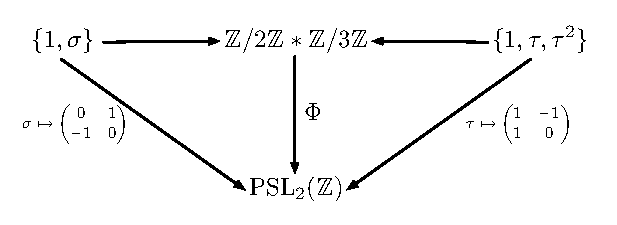
\includegraphics{grugraImages/PSL}
\end{center}
Der Nachweis, dass $\Phi$ in der Tat ein Isomorphismus ist, ist nicht
trivial.

\BEM Die Konstruktion der freien Produkte lässt sich
ohne Weiteres auf beliebige Indexmengen $I$ verallgemeinern:
\begin{enumerate}
\item Es seien $(G_i)_{i\in I}$ Gruppen. Dann gibt es eine (bis auf
Isomorphie) eindeutige Gruppe $G=*_{i\in I} G_i$ und
Gruppenhomomorphismen $\alpha_i:G_i\Ra G$, so dass
für eine Gruppe $H$ und Homomorphismen $\phi_i:G_i\Ra H$
ein eindeutiger Homomorphismus $\Phi:G\Ra H$ existiert mit
$\Phi\circ\alpha_i=\phi_i$ für alle $i\in I$.
\item Ist $G_i=\lag S_i|R_i\rag$, so ist
$G=\lag \os{\bigcup}{.}_{i\in I}S_i|\os{\bigcup}{.}_{i\in I}R_i \rag$.
\item $G$ ist die Menge aller reduzierten Wörter über
$\os{\bigcup}{.}_{i\in I} G_i$, bei denen aufeinanderfolgende
Buchstaben aus verschiedenen $G_i$ kommen.
\end{enumerate}

\BEM\label{bem_freiprodukt}
Durch die Inklusionen
\begin{align*}
\iota_1:G_1\Ra G_1\times G_2,\quad g\mapsto(g,1) \\
\iota_2:G_2\Ra G_1\times G_2,\quad h\mapsto(1,h)
\end{align*}
ist über die UAE des freien Produktes ein Gruppenhomomorphismus
\[
\rho:G_1*G_2\Ra G_1\times G_2
\]
gegeben. Es gilt:
\begin{enumerate}
\item
\begin{align*}
\rho(g_1 h_1\cdots g_n h_n) &=
\rho(g_1)\rho(h_1)\cdots\rho(g_n)\rho(h_n) \\
&=\rho\circ\alpha_1(g_1)\rho\circ\alpha_2(h_1)\cdots\rho\circ\alpha_1(g_n)\rho\circ\alpha_2(h_n) \\
&=\iota_1(g_1)\iota_2(h_1)\cdots\iota_1(g_n)\iota_2(h_n) \\
&=(g_1,1)(1,h_1)\cdots(g_n,1)(1,h_n) \\
&=(g_1\cdots g_n,h_1\cdots h_n).
\end{align*}
\item $\rho$ ist surjektiv, also
\[
G_1\times G_2 \cong G_1*G_2/\K{\rho}.
\]
\item $\K{\rho}$ ist eine freie Gruppe mit Basis
\[
X=\{ ghg^{-1}h^{-1}:g\in G_1\backslash\{1\},h\in G_2\backslash\{1\}\}.
\]
\end{enumerate}
In Buch von Serre \cite{serre} wird ein elementarer Beweis hierfür
gebracht, den wir kurz nun skizzieren:
Zuerst rechnet man leicht nach, dass $K:=\lag X\rag$ ein Normalteiler
und im Kern von $\rho$ enthalten ist, d.h. es gibt ein $\tilde{\rho}$,
so dass
\[\xymatrix{
G_1*G_2 \ar[r]^{\rho}\ar[d] & G_1\times G_2 \\
G_1*G_2/K \ar[ur]_{\tilde{\rho}}
}\]
kommutiert. Zeigt man nun, dass $\tilde{\rho}$ ein Isomorphismus
(mit Umkehrabbildung $(g,h)\mapsto gh K$) ist, so folgt
$\K{\rho}=K$. Nun muss noch gezeigt werden, dass der Kern frei ist.

Später werden wir einen anderen Beweis für diese Bemerkung geben.